\documentclass[tikz]{standalone}
\usepackage{pgfplots}
\pgfplotsset{compat=1.15}
\usepackage{mathrsfs}
\usetikzlibrary{arrows,calc}
\usepackage{tkz-euclide}

\usepackage{fp}
\pagestyle{empty}

\definecolor{AngleClr}{rgb}{0,0.39215686274509803,0}
\definecolor{ShapeClr}{rgb}{0.6,0.2,0}

\begin{document}

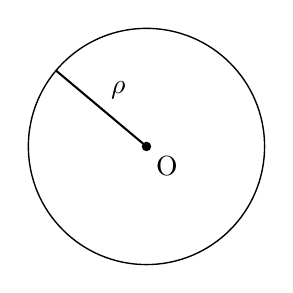
\begin{tikzpicture}[scale=.75]
\tkzSetUpLine[line width=1pt,color=black]
\tkzSetUpPoint[fill=black]

\tkzDefPoints{0/0/O,2/0/X}

\tkzDefPoint(140:2){A}

\tkzDrawCircle[color=black,line width=0.5pt,fill=white](O,X)
\tkzDrawSegments[line width=0.75pt](O,A)

\tkzDrawPoints[size=3](O)

\tkzLabelPoint[below right](O){$\rm O$}
\tkzLabelSegment[above right](O,A){$\rho$}


\end{tikzpicture}

\end{document}
